\documentclass[a4paper,12pt]{article}
\usepackage{a4wide}
\usepackage[pdftex]{hyperref}
\usepackage[german]{babel}
\usepackage[utf8]{inputenc}
\usepackage{amssymb}
\usepackage{csquotes}
\usepackage{wrapfig}
\usepackage{graphicx}
\usepackage{multicol}
\usepackage{amsmath}
\usepackage{enumitem}
\usepackage{polynom}
\usepackage{siunitx}

\setlength{\marginparsep}{1 cm}
\setlength{\topmargin}{-0.6in}
\setlength{\textheight}{9.5in}
\pagestyle{plain}

\polyset{%
   style=C,
   delims={\big(}{\big)},
   div=:
}

% Polynomial long division
\polyset{%
	style=C,
	delims={\big(}{\big)},
	div=:
}

% Differential operator
\newcommand{\diff}[1]{\:\mathrm{d}{#1}}
\newcommand{\pdd}[2]{\frac{\partial #1}{\partial #2}}
\newcommand{\pddn}[3]{\frac{\partial^{#1} #2}{\partial #3^{#1}}}
\newcommand{\dd}[2]{\frac{\mathrm{d}{#1}}{\mathrm{d}{#2}}}
\newcommand{\ddn}[3]{\frac{\mathrm{d}^{#1}{#2}}{\mathrm{d}{#3^{#1}}}}

% N-th root
% \nroot{3}{27}
\newcommand*{\nroot}[2]{\sqrt[\leftroot{-1}\uproot{2}#1]{#2}}
\newcommand*{\ncroot}[4]{\sqrt[\leftroot{#1}\uproot{#2}#3]{#4}}

% 2 component vector
% \tvect{1}{-1}
% \tvec{1}{-1}
\newcommand{\tvect}[2]{%
   \ensuremath{\Bigl(\negthinspace\begin{smallmatrix}#1\\#2\end{smallmatrix}\Bigr)}}
\newcommand{\tvec}[2]{%
    \ensuremath{\left(\negthinspace\begin{matrix}#1\\#2\end{matrix}\right)}}

% 3 component vector
% \rvect{1}{-1}{0}
% \rvec{1}{-1}{0}
\newcommand{\rvect}[3]{%
   \ensuremath{\Bigl(\negthinspace\begin{smallmatrix}#1\\#2\\#3\end{smallmatrix}\Bigr)}}
\newcommand{\rvec}[3]{%
    \ensuremath{\left(\negthinspace\begin{matrix}#1\\#2\\#3\end{matrix}\right)}}

% Long vector arrow
% \xshlongvec{ABC}

% German-style quotation marks %
\MakeOuterQuote{"}

% Number sets
\newcommand{\N}{\mathbb{N}}
\newcommand{\Z}{\mathbb{Z}}
\newcommand{\Q}{\mathbb{Q}}
\newcommand{\R}{\mathbb{R}}
\newcommand{\C}{\mathbb{C}}

\newcommand{\setzero}{\varnothing}

% Mention (small caps)
\newcommand{\mention}[1]{\textsc{#1}}

% Functions
\newcommand{\asin}[0]{\text{asin}}
\newcommand{\acos}[0]{\text{acos}}
\newcommand{\atan}[0]{\text{atan}}
\newcommand{\sgn}[0]{\text{sgn}}
\newcommand{\grad}[0]{\text{grad}}

% Scale
% Usage in math mode: \Scale[1.5]{...equation...} %
\newcommand*{\Scale}[2][4]{\scalebox{#1}{$#2$}}%

% Units
\newcommand{\um}{\text{m}}
\newcommand{\us}{\text{s}}
\newcommand{\ukm}{\text{km}}
\newcommand{\ukg}{\text{kg}}
\newcommand{\uh}{\text{h}}
\newcommand{\ukmh}{\frac{\ukm}{\uh}}
\newcommand{\umpers}{\frac{\um}{\us}}
\newcommand{\umss}{\frac{\ukm}{\us^2}}
\newcommand{\ukgss}{\frac{\ukg}{\us^2}}
\newcommand{\degrees}[1]{\SI{#1}{\degree}}

% Floor / ceil
\newcommand{\floor}[1]{\left\lfloor #1 \right\rfloor}
\newcommand{\ceil}[1]{\left\lceil #1 \right\rceil}

% Circle characters
\newcommand*\circled[1]{
    \tikz[baseline=(char.base)]{
        \node[shape=circle,draw,inner sep=2pt] (char) {#1};
    }
}



\begin{document}

\begin{center}
{\bf {\large Aufgabenblatt 7 MI/IT}}
\end{center}

\begin{enumerate}

\item Klassifizieren Sie die folgenden DGL bezüglich der im Unterricht besprochenen Merkmale. [Zusatz] Überlegen Sie sich durch geschicktes Nachdenken eine Funktion, welche die DGL erfüllt.

\begin{multicols}{3}
\begin{enumerate}
\item $y'(x) = x$
\item $y'(x) =  e^x$
\item $y'(x)= 2\cdot y(x)$
\item $y''(x) = 42$
\item $ y''(x) = y(x)$
\item $y'(x) = \frac{1}{y(x)}$
\end{enumerate}
\end{multicols}



\item Klassifizieren Sie die DGL! Vorgegeben ist die allgemeine Lösung der DGL. Finden Sie eine partikuläre Lösung, welche die gegebene Anfangsbedingung erfüllt!

\begin{enumerate}
\item{$y' = x$ mit Lösung $y=\frac{1}{2}x^2+C$ für $y(0)=4$}
\item{$y' = y$ mit Lösung $y=C\cdot e^x$ für $y(0)=4$}
\item{$y' = 3y$ mit Lösung $y=C \cdot e^{3x}$ für $y(0)=4$ }
\item{$y'' = 3y$ mit Lösung $y=C_1 e^{\sqrt{3}x} + C_2 e^{-\sqrt{3}x}$ für $y(0)=4$ und $y'(0)=5$}
\item{$y'' = -3y$ mit Lösung $y=C_1 \cos(\sqrt{3}\cdot x) + C_2 \sin(\sqrt{3}\cdot x)$ für $y(0)=4$, $y'(0)=5$}
\end{enumerate}



\item

In einen undichten Tank fließen pro Sekunde 10~l Wasser. Außerdem sickert jede Sekunde ein Promille der aktuellen Wassermenge aus dem Tank. Zum Zeitpunkt $t=7\,\mbox{s}$ enthält der Tank 98~l. Der Tank sei so groß ist, dass er nie voll wird. Stellen Sie eine Differentialgleichung für die Wassermenge im Tank auf und geben Sie die Anfangsbedingung an. Schreiben Sie alle Zahlenwerte mit ihren physikalischen Einheiten auf! Klassifizieren Sie diese DGL!


\item Prüfen Sie, ob die folgende DGL homogen und linear sind ! Falls nichts, geben Sie den homogenen und den inhomogenen Anteil an!

\begin{multicols}{3}
	\begin{enumerate}
		\item $y'=y$
		\item $y'=y+\sin(x)$
		\item $x^2y''=2y'-y$
		\item $0=\frac{y''+2y}{y'''-3y}$
		\item $\frac{y'}{y}=(x+\frac{1}{y})$
		\item $(y'')^2=\ln(x)(yy')$
		\item $\sqrt{y'+y}=0$
		\item $y''-2y'+y=\sin(x)$
		\item $\ln(x)y''+\frac{y'}{x}=0$
	\end{enumerate}
\end{multicols}


\begin{center}
(bitte wenden)
\end{center}

\newpage

\item Wir betrachten die DGL $yy'+x-2y'=3$ und wollen das Richungsfeld skizzieren, für x- und y-Werte im Intervall $[0,5]$.
\begin{enumerate}
\item Formen Sie die DGL in explizite Form um, d.h. stellen Sie um nach $y'$.
\item Für das Richtungsfeld ist der Anstieg an verschiedenen Punkten zu berechnen. Um die Arbeit zu verringern, betrachten wir, an welchen Stellen der Anstieg $y'$ konstant ist. Dort zeigt das Richtungsfeld in die gleiche Richtung. Stellen Sie die Gleichung $y'=c$ (c: beliebige Konstante) nach $y(x)$ um.
\item Zeichnen Sie die so erhalten Funktionen $y(x)$ für $c\in\lbrace-5;-2;-0.5,-0,1;1,5\rbrace$. Zeichnen Sie zudem das Richtungfeld entlang diesen Funktionen. Anmerkung: Kurven, auf denen $y'=const$ gilt, nennt man Isoklinen (von lat. in\textbf{clin}are, engl. in\textbf{clin}ation, "Neigung").
\item Ermitteln Sie graphisch die Lösung der DGL für $(i)$ das Anfangswertproblem $y(4)=2$ und $(ii)$ für das Anfangswertproblem $y(1) = 1$. Um was für ein geometrisches Objekt handelt es sich bei den Lösungen?
\item Veranschaulichen Sie sich die Lösung mittels dem Online-Tool \href{https://www.geogebra.org/m/W7dAdgqc}{Geogebra}. Für den Anfangswert $y(2)=3$ zeigt dieses Tool (s. Abbildung \ref{ex-ode-slope-field-1-img-a}) links und rechts unerwartete Sprünge. Können Sie sich dieses Verhalten erklären? (Hinweis: Die Gleitkommazahlen stellen eine abzählbare, endliche Menge dar.)
\end{enumerate}


\begin{figure}[ht]
	\centering
	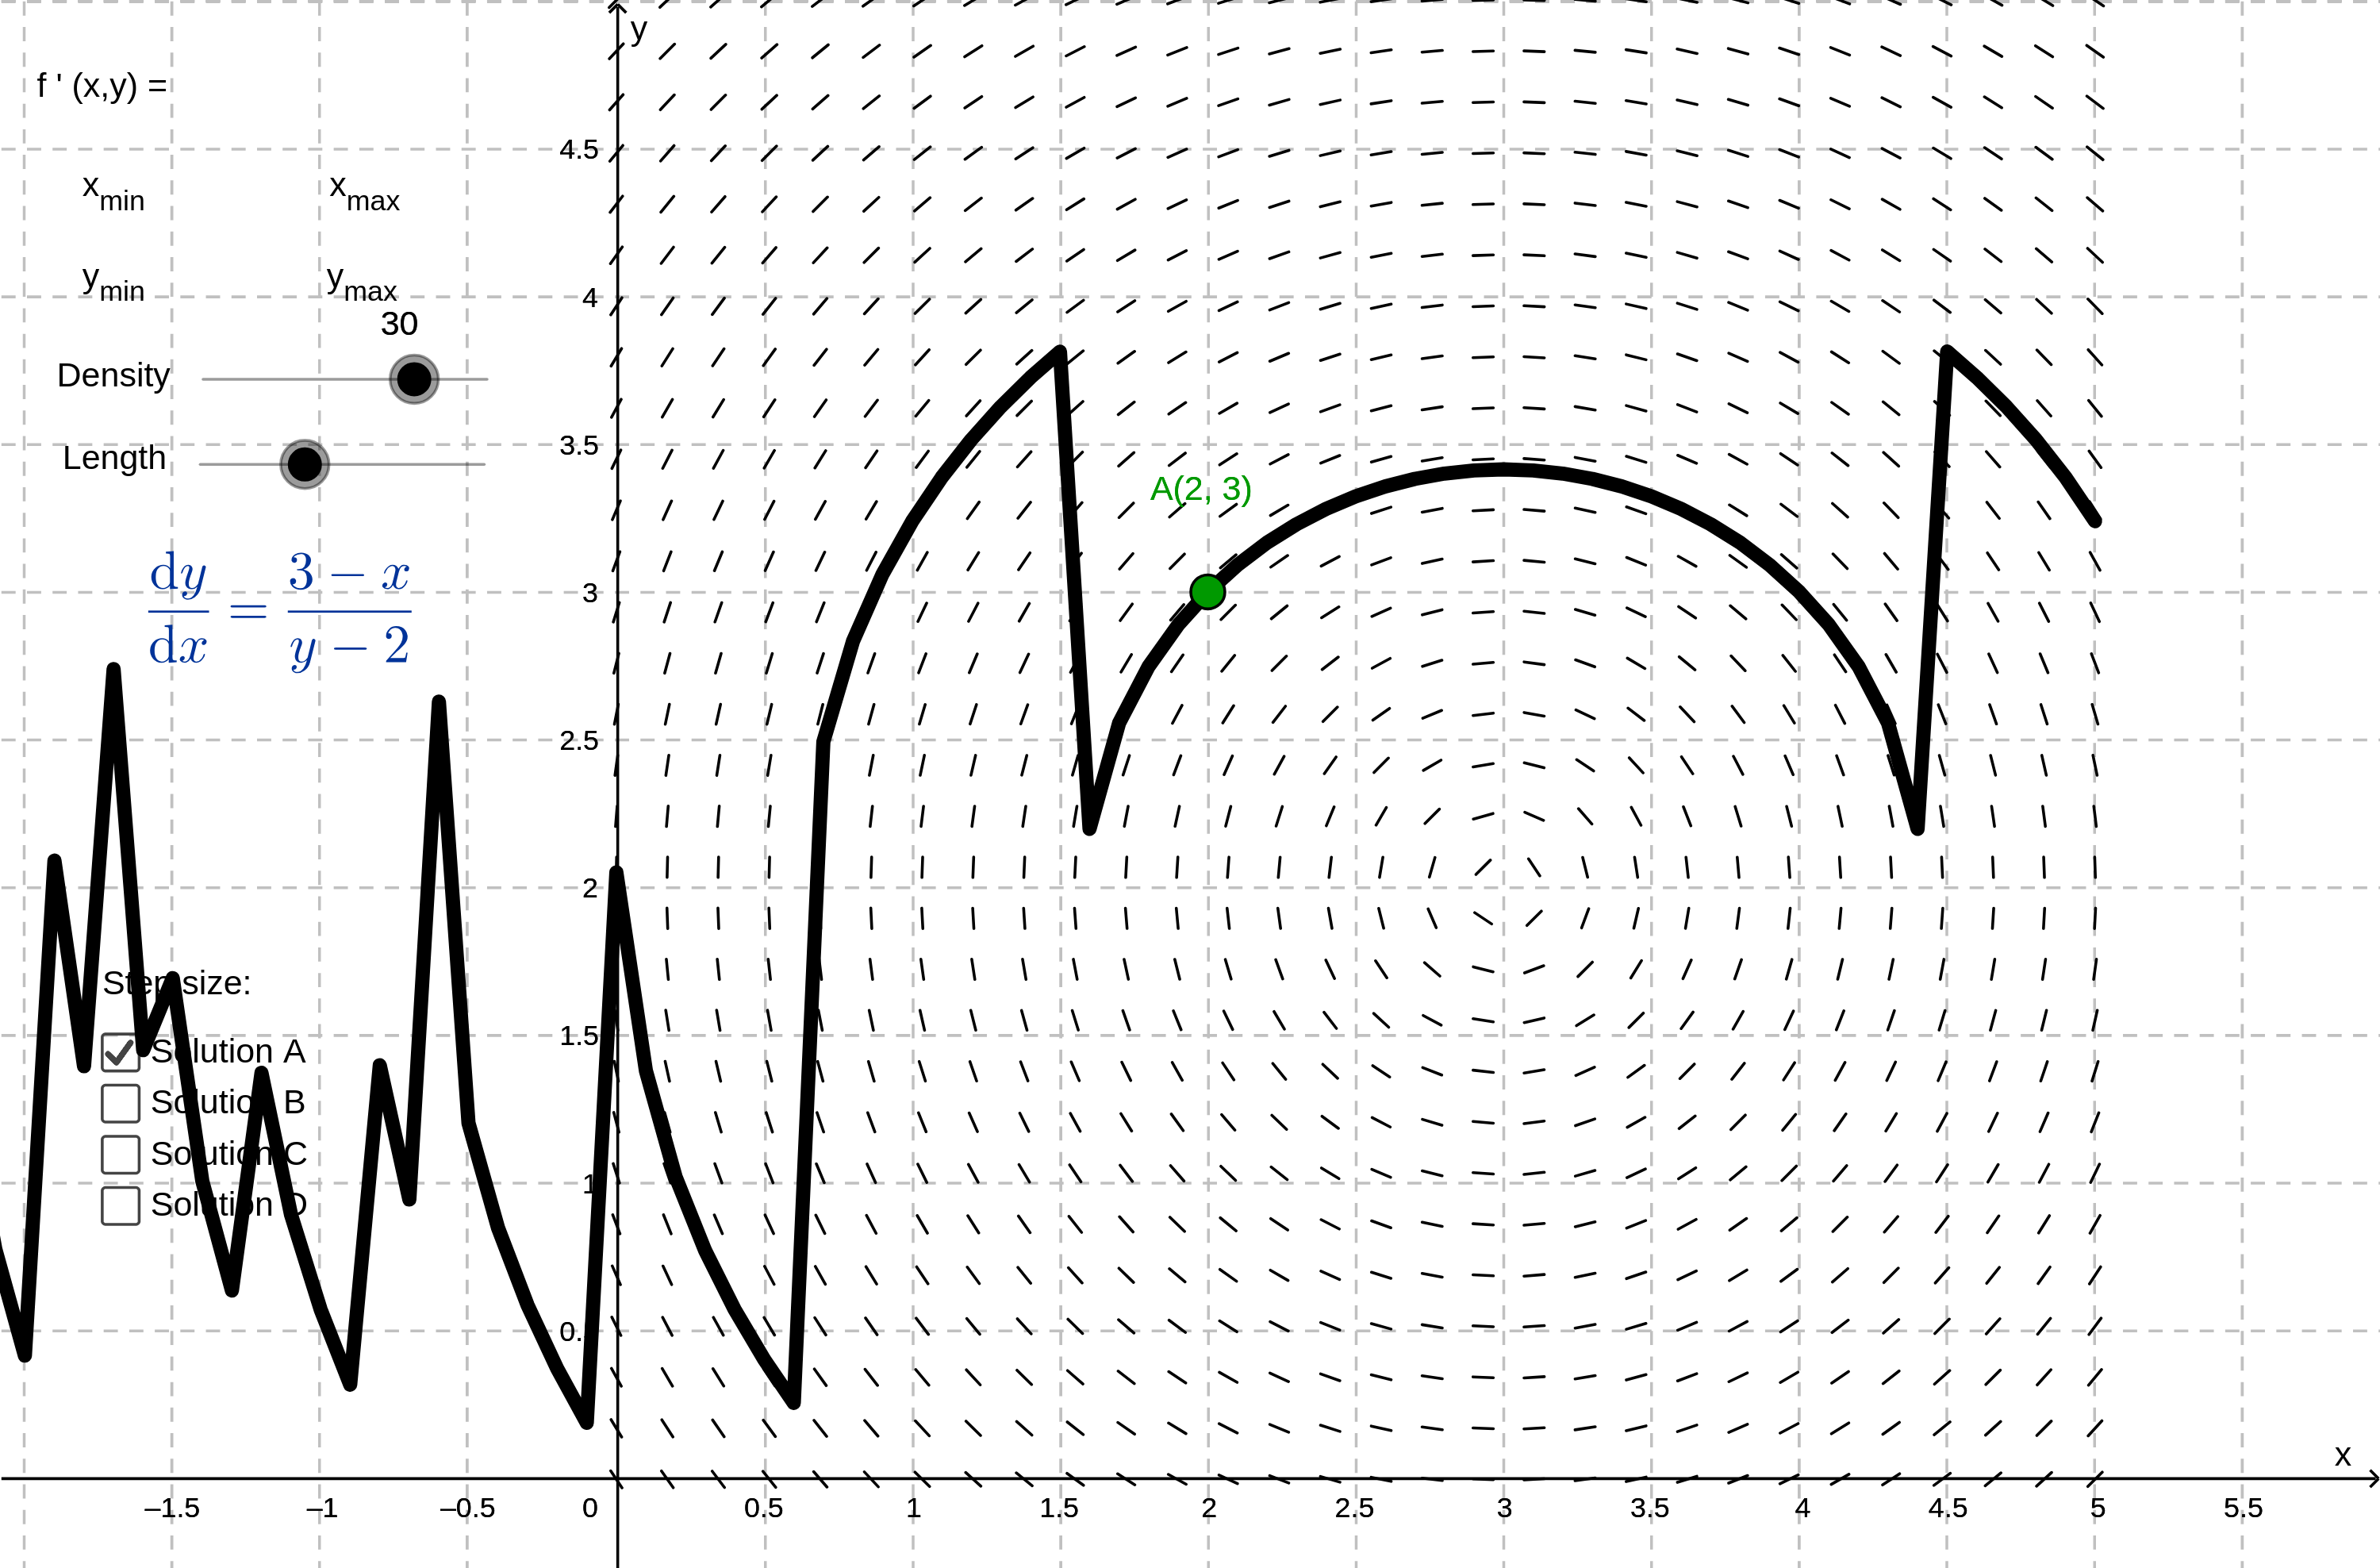
\includegraphics[width=0.45\textwidth]{../pool/ex-ode-slope-field-1-img-a.png}
	\caption{Numerische Lösung der DGL aus Aufgabe 1.5 mittels Geogebra für den Anfangswert $y(2)=3$. (https://www.geogebra.org/m/W7dAdgqc)}.
	\label{ex-ode-slope-field-1-img-a}
\end{figure}



Rätselaufgabe:
Wie tief ist der See? (s. Abbildung \ref{ex-trigonometry-1-img-a})
\noindent
"Nehmen wir an, die Wasserlilie ragte, wie in unserer Zeichnung, 10 Zoll über die Oberfläche hinaus und verschwände darunter, wenn man sie zur Seite ziehen würde, 21 Zoll von ihrem ursprünglichen Standort entfernt. Wie tief ist dann das Wasser?" (Mathematische Rätsel und Spiele, Der Klassiker, Sam Loyd, Martin Gardner)

\end{enumerate}

\begin{figure}[ht]
	\centering
	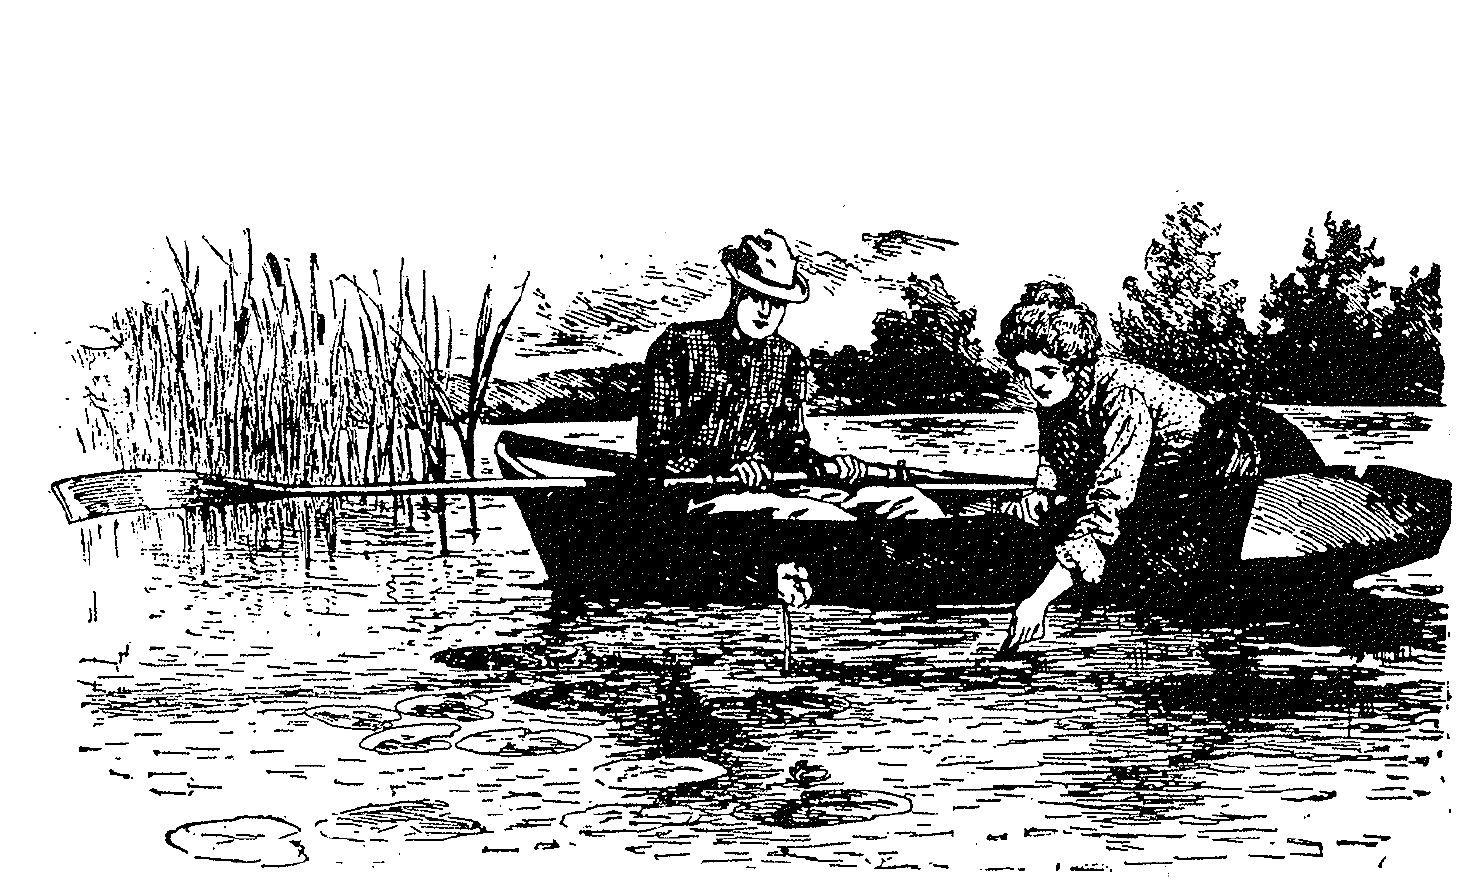
\includegraphics[width=0.45\textwidth]{../tex-snippets/ex-trigonometry-1-img-a.png}
	\caption{Skizze zur Rätselaufgabe über die Wasserlilie}.
	\label{ex-trigonometry-1-img-a}
\end{figure}



\newpage

\begin{center}
{\bf {\large Lösungen}}
\end{center}

\begin{enumerate}

\item

\begin{enumerate}
\item Ordnung 1, gewöhnlich, explizit. Inhomogen, homogener Anteil $y'=0$ hat Grad 1, also linear.

Direkte Integration liefert $y = \int x \d x = \frac{1}{2}x^2+C$

\item Ordnung 1, gewöhnlich, explizit. Inhomogen, homogener Anteil $y'=0$ hat Grad 1, also linear.

Direkte Integration liefert $y = \int e^x \d x = e^x + C$.

\item Ordnung 1, gewöhnlich, explizit. Homogen mit Grad 1, also linear.

Gesucht ist eine Funktion, deren Ableitung gleich dem Doppelten der Funktion ist. Die Exponentialfunktion $y = e^x$ ändert sich nicht, wenn man sie ableitet. Multiplizieren wird das Argument mit einem Faktor, wandert dieser beim Ableiten nach der Kettenregel als Koeffizient vor die Expoentialfunktion. Also ist $y = e^{2x}$ eine Lösung der DGL. Zudem können wir die Exponentialfunktion auch mit einem beliebigen Faktor multiplizieren, dieser wird beim Ableiten übernommen. Die allgemeine Lösung ist daher $y = C\cdot e^{2x}$.

\item Ordnung 2, gewöhnlich, explizit. Inhomogen mit homogenen Anteil $y''=0$, dieser hat Homogenitätsgrad 1, also linear.

Zweifache direkte Integration liefert:

$$y = \int \int 42 \d x \d x = \int 42x +C_1 \d x = 21x^2 + C_1 x + C_2$$

\item Ordnung 2, gewöhnlich, explizit. Homogen vom Grad 1, also linear

Wir suchen eine Funktion, deren zweite Ableitung der Funktion selbst entspricht. Wir wissen, dass die Exponentialfunktion $y=e^{ax}$  dies für $a=1$ erfüllt. Wir möchten wissen, ob dies auch für andere Werte von $a$ gilt. Es gilt $y'' = a^2 e^{ax}$. Durch Einsetzen des Ansatzes $y=e^{ax}$ in die DGL erhalten wir:

$$a^2 e^{ax} = e^{ax}$$
$$\implies a^2 = 1$$
$$\implies a = \pm 1$$

Somit lauten zwei Lösungen $y_1 = e^x$ und $y_2 = e^{-x}$. Die allgemeine Lösung der DGL ist gegeben durch $y = C_1 e^x + C_2 e^{-x}$ (durch Probe bestätigen!).

\item Ordnung 1. gewöhnlich, explizit. Umschreiben als $y'y-1=0$. Inhomogen, der homogene Anteil ist $y'y=0$ mit Grad der Homogenität 2, also nichtlinear.

Gesucht ist eine Funktion, deren Kehrwert gleich ihrer Ableitung ist. Funktionen wie $y = \ln(x)$ oder $y = \sin(x)$ scheiden aus, da sie beim Ableiten in ganz andere Funktionen übergehen. Die Ableitung der Potenzfunktion $y=x^n$ ist $y' = n x^{n-1}$. Potenzen mit negativen Exponenten lassen sich schreiben als Brüche, also $x^{-a} = \frac{1}{x^a}$

Wenn wir also für $n=\frac{1}{2}$ wählen, dann ist die Ableitung auch eine Potenzfunktion mit dem betragsmäßig gleichen Exponenten: $y=x^{\frac{1}{2}}$ mit der Ableitung $y'=\frac{1}{2}\cdot\frac{1}{x^\frac{1}{2}}$.

Dies erfüllt aufgrund des Vorfaktors $\frac{1}{2}$ noch nicht die DGL. Wir versuchen, den Ansatz noch mit einer Konstante zu multiplizieren: $y=a x^{\frac{1}{2}}$. Die Ableitung ist dann $y'=\frac{1}{2}ax^{-\frac{1}{2}}$. Der Kehrwert des Ansatzes beträgt $1/y = \frac{1}{a} x^{-\frac{1}{2}}$. Damit $y' = 1/y$ gilt, muss demzufolge $\frac{1}{2}a = \frac{1}{a}$ gelten, also $a^2 = 2$. Somit ist $a=\pm \sqrt{2}$ und zwei Lösungen der DGL sind $y=\pm\sqrt{2}\cdot\sqrt{x}$.

Hinweis: Die allgemeine Lösung findet man durch Trennung der Variablen:

$$\frac{\d y}{\d x} = \frac{1}{y}$$
$$\implies \int y \d y = \int \d x$$
$$\implies \frac{y^2}{2} = x + C$$
$$\implies y = \pm\sqrt{2}\cdot\sqrt{x+C}$$
\end{enumerate}



\item

\begin{enumerate}
\item Ordnung 1, gewöhnlich, explizit, inhomogen, linear

Direkte Integration liefert die allgemeine Lösung $y=\frac{x^2}{2}+C$. Die Anfangsbedingung ausgewertet ergibt $y(0)=\frac{0^2}{4}+C=4$, also $C=4$. Somit ist die partikuläre Lösung $y=\frac{x^2}{2}+4$.

\item Ordnung 1, gewöhnlich, explizit, homogen, linear

Die allgemeine Lösung lautet $y=C e^x$. Die Anfangsbedingung ergibt $y(0)=C\cdot e^0 = C = 4$. Somit ist die partikuläre Lösung $y=4e^x$.

\item Ordnung 1, gewöhnlich, explizit, homogen, linear

Die allgemeine Lösung lautet $y=C e^{3x}$. Die Anfangsbedingung ergibt $y(0)=C\cdot e^0 = C = 4$. Somit ist die partikuläre Lösung $y = 4 e^{3x}$.

\item Ordnung 2, gewöhnlich, explizit, homogen, linear

$y''-3y=0$. Die zugehörige charakteristische Gleichung lautet $\lambda^2-3 = 0$ und hat die Lösungen $\lambda = \pm \sqrt{3}$. Die allgemeine Lösung lautet mithin

$$y=C_1 e^{\sqrt{3}x} + C_2 e^{-\sqrt{3}x}$$

Für die Anfangsbedingungen benötigen wir noch die 1. Ableitung, diese lautet:

$$y'= C_1 \sqrt{3} e^{\sqrt{3}x} - C_2 \sqrt{3} e^{-\sqrt{3}x}$$

Nun können wir die Anfangsbedingungen einsetzen und erhalten:

$$y(0) = 4 = C_1 + C_2$$
$$y'(0) = 5 = C_1 \sqrt{3} - C_2 \sqrt{3}$$

Dies stellt ein lineares Gleichungssystem dar. Zur Lösung multiplizieren wir die erste Gleichung mit $\sqrt{3}$ und addieren dazu die zweite Gleichung:

$$\sqrt{3}y(0)+y'(0) = 4\sqrt{3} + 5 = 2\sqrt{3}C_1$$
$$\implies C_1 = 2 + \frac{5}{2\sqrt{3}} = 2 + \frac{5}{6}\sqrt{3}$$

Für die andere Konstante folgt somit

$$C_2 = 4 - C_1 = 2 - \frac{5}{6}\sqrt{3}$$

Damit lautet die partikuläre Lösung:

$$y = (2 + \frac{5}{6}\sqrt{3}) e^{\sqrt{3}x} + (2 - \frac{5}{6}\sqrt{3}) e^{-\sqrt{3}x}$$

\item Ordnung 2, gewöhnlich, explizit, homogen, linear

$y''+3y = 0$. Die charakteristische Gleichung lautet $\lambda^2+3 = 0$ und hat die Lösungen $\lambda = \pm \sqrt{3} j$. Die allgemeine Lösung im Reellen lautet damit

$$y = C_1 \cos(\sqrt{3}x) + C_2 \sin(\sqrt{3}x)$$

Die Ableitung lautet:

$$y' = - C_1 \sqrt{3} \sin(\sqrt{3}x) + C_2 \sqrt{3} \cos(\sqrt{3}x)$$

Die Anfangsbedingungen ergeben:

$$y(0) = 4 = C_1$$
$$y'(0) = 5 = C_2 \sqrt{3}$$

Somit ist die partikuläre Lösung:

$$y = 4 \cos(\sqrt{3}x) + \frac{5}{3}\sqrt{3} \sin(\sqrt{3}x)$$

\end{enumerate}



\item

Die Wassermenge (in Litern) im Tank sei bezeichnet mit $V$. Die Zuflussrate beträgt $\sigma_z = 10 \frac{l}{s}$ (Liter pro Sekunde). Die Abflussrate ist $\sigma_a = -\frac{1}{1000} V$ (Promille = pro Mille(Tausend) = 1 Tausendstel).

Zu jedem Zeitpunkt setzt sich die Änderung $dV$ der Wassermenge zusammen aus Zufluss- und Abflussrate:

$$\dd{V}{t} = V'(t) = \sigma_z + \sigma_a = \sigma_z - \frac{1}{1000}V$$
$$\implies V' + \frac{1}{1000} V = \sigma_z = 10 \frac{l}{s}$$

Es handelt sich um eine DGL vom Ordnung 1, gewöhnlich, explizit, inhomogen, linear.

Bei 7 Sekunden enthält der Tank 98 Liter. Die Anfangsbedingung lautet also:

$$V(7s) = 98l$$



\item Zuerst alle Terme auf eine Seite bringen, dann die Definition von Homogenität anwenden.

\begin{enumerate}

\item $\phi(y,y',x) = y'-y = 0$ ist homogen vom Grad $1$, denn:

$$\phi(ty,ty',x) = (ty)'-(ty) = t^1\cdot(y'-y) = t^1\cdot\phi(y,y',x))$$

\item $\phi(y,y',x) = y'-y-\sin(x) = 0$ ist inhomogen, denn:

$$\phi(ty,ty',x) = (ty)'-(ty)-\sin(x) = t^1 \cdot(y'-y) -\sin(x) \ne t^1\cdot\phi(y,y',x))$$

Die zugehörige homogene DGL ist $\phi_h = y'-y = 0$, die Inhomogenität ist $\psi=-\sin(x)$.

\item Die DGL $x''y''-2y'+y=0$ ist homogen vom Grad $1$, denn:

$$x''(ty)''-2(ty)'+(ty) = t^1\cdot(x''y''-2y'+y)$$

\item Die DGL $0=\frac{y''+2y}{y'''-3y}$ ist homogen vom Grad $0$, denn (beachte, dass $t^0=1$):

$$\frac{(ty)''+2(ty)}{(ty)'''-3(ty)} = \frac{t(y''+2y)}{t(y'''-3y)} = t^0 \frac{y''+2y}{y'''-3y}$$

\item Die DGL $y'-xy-1=0$ ist inhomogen, denn:

$$(ty)'-x(ty)-1=t^1 (y'-xy)-1 \ne t^1 (y'-xy-1)$$

Die zugehörige homogene DGL ist $\phi_h = y'-xy=0$, die Inhomogenität ist $\psi = -1$.

\item Die DGL $(y'')^2-\ln(x)(yy') = 0$ ist homogen vom Grad $2$, denn:

$$((ty)'')^2-\ln(x)((ty)(ty)') = t^2\cdot((y'')^2-\ln(x)(yy'))$$

\item Die DGL $\sqrt{y'+y}=0$ ist homogen vom Grad $\frac{1}{2}$, denn:

$$\sqrt{(ty)'+(ty)} = \sqrt{t(y'+y)} = t^{\frac{1}{2}}\sqrt{y'+y}$$

\end{enumerate}



\item

\begin{enumerate}
\item Durch identisches Umformen erhalten wir:

$$y'(y-2) = 3-x$$
$$\implies y' = \frac{3-x}{y-2}$$

\item Wir stellen für ein $c \in \mathbb{R}$ um:

$$y' = \frac{3-x}{y-2} = c$$
$$\implies y-2 = \frac{3-x}{c}$$
$$\implies y(x) = \frac{3-x}{c}+2$$
$$\implies y(x) = -\frac{1}{c}(x-3)+2$$

Es handelt sich bei den Isoklinen also um Geraden mit dem Anstieg $-\frac{1}{c}$, welche um $2$ Einheiten nach oben und um $3$ Einheiten nach rechts verschoben sind. Alle Isoklinen verlaufen durch den Punkt $(3,2)$.

\item Auf jedem Punkt einer solchen Gerade ist der Anstieg gleich. Der einzuzeichnende Anstieg des Richtungsfelds ist $c$, der zugehörige Anstieg der Isoklinen $m'=-\frac{1}{c}$. Es gilt daher $m'\cdot c = -1$, also steht der einzuzeichnende Anstieg orthogonal (senkrecht) zur Isoklinen.

\item Anders gesagt sind die Isoklinen daher Strahlen, welche radial vom Punkt $(3,2)$ ausgehen. Die Lösungskurven verlaufen senkrecht dazu, es handelt sich mithin um alle Kreise mit dem Ursprung $(3,2)$. Für den Anfangswert $y(4)=2$ beträgt der Radius des Kreises $r_{4,2} = \sqrt{(4-3)^2+(2-2)^2} = 1$, für $y(1)=1$ beträgt er $r_{4,2} = \sqrt{(1-3)^2+(1-2)^2} = \sqrt{5}$.

\item Das Online-Tool verwendet sogenannte numerische Lösungsverfahren, welche die wahre Lösungsfunktion aufgrund der Beschränktheit der Gleitkommazahlen nur approximativ (näherungsweise) ermitteln können. Ein einfaches solches Näherungsverfahren besteht darin, vom durch den Anfangswert gegebenen Punkt auszugehen (vgl. Abbildung \ref{fig4}). In finiten Schritten $\Delta x$ wird dann entsprechend dem momentanten Anstieg nach links bzw. nach rechts geschritten. Wo die Sprünge zu sehen sind, ist der Betrag des Anstiegs $|y'|$ sehr groß, sodass auch der Fehler bei einem Schritt $\Delta x$ größer wird. Am linken bzw. rechten Punkt des Kreises ist der Anstieg nicht mehr endlich, hier versagt das einfache Lösungsverfahren.

\end{enumerate}


\begin{figure}[ht]
	\centering
	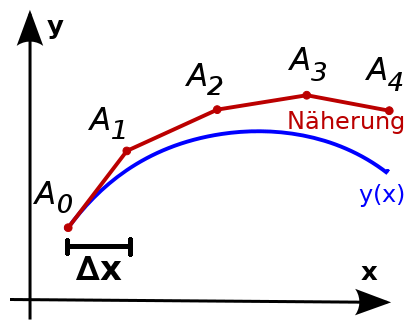
\includegraphics[width=0.4\textwidth]{../tex-snippets/ex-ode-slope-field-1-img-b.png}
	\caption{Einfaches numerisches Lösungsverfahren einer DGL der Ordnung 1 (Eulerverfahren). Es wird in endlich Schritten $\Delta x$ mit dem jeweiligen Anstieg von $A_0$ nach rechts zu $A_4$ geschritten. Die so erhaltene Kurve (rot) weicht von der tatsächlichen Lösungskurve (blau) ab. Je größer der Anstieg der Lösungskurve, desto größer ist der Fehler bei gegebenen $\Delta x$.}
	\label{ex-ode-slope-field-1-img-b}
\end{figure}



\item Siehe Skizze \ref{ex-trigonometry-1-img-b}. Wir erhalten die beiden Gleichungen:

\begin{alignat*}{3}
(i)  \;  & L \cdot \cos(\alpha)  &&= L - h \\
(ii) \; &  L \cdot \sin(\alpha)  &&= w
\end{alignat*}

($w=21cm$, $h=10cm$, $\alpha$: Winkel zwischen der Senkrechten und der geneigten Lilie, $L$: gesuchte Tiefe des Sees)

Zur Lösung bilden wir die Summe der Quadrate beider Gleichungen:

$$(i)^2+(ii)^2 = L^2 (\cos^2(\alpha) + \sin^2(\alpha)) = (L-h)^2 + w^2$$

Da nun $\cos^2(\alpha) + \sin^2(\alpha) = 1$ gilt (Satz des Pythagoras)

$$ L^2 = L^2 + h^2 - 2Lh + w^2$$
$$\implies 0 = h^2-2Lh+w^2$$
$$\implies L = \frac{h^2+w^2}{2h}$$

Wir setzen die gegebenen Werte ein und erhalten für die Tiefe des Sees:

$$L=\frac{10^2\cdot\text{inch}^2 + 21^2\cdot\text{inch}^2}{2\cdot 10 \cdot\text{inch}} \approx 27,0 \text{ inch} = 69 \text{ cm}$$

Der Neigungswinkel beträgt dann $\alpha = \arcsin(\frac{w}{L})= \arcsin(\frac{21}{69}) \approx 17,7 ^ \circ$.

\begin{figure}[ht]
	\centering
	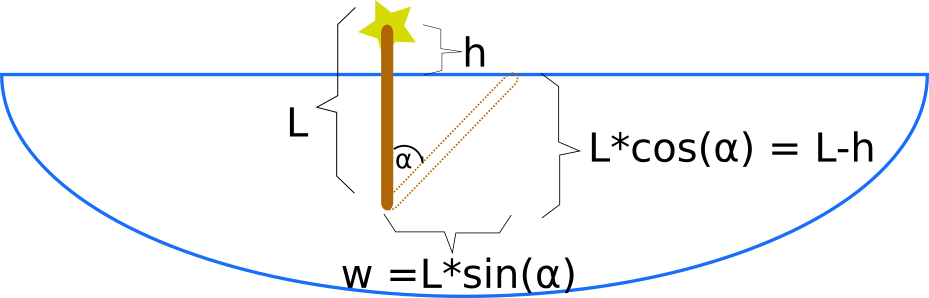
\includegraphics[width=0.75\textwidth]{../pool/ex-trigonometry-1-img-b.png}
	\caption{Skizze zur Rätselaufgabe.}
	\label{ex-trigonometry-1-img-b}
\end{figure}



\end{enumerate}

\end{document}

